\documentclass[11pt]{article}
\usepackage[margin=1in]{geometry}
\usepackage{amsmath,amssymb}
\usepackage{enumitem}
\usepackage{hyperref}
\usepackage{graphicx}
\usepackage{booktabs}
\usepackage{parskip}
\usepackage{float}
\usepackage{subcaption}
\usepackage[T1]{fontenc}
\usepackage[utf8]{inputenc}
\usepackage{lmodern}
\usepackage{xcolor}

\hypersetup{colorlinks=true, linkcolor=blue, urlcolor=blue, citecolor=blue}
\graphicspath{{figures/}}

\title{Formal RL Length Generalization: GRPO Process-Reward Analysis on Parity}
\author{Ravi Raj Kumar}
\date{June 2026}

\begin{document}
\maketitle

\begin{abstract}
This report summarizes the current \texttt{formal\_rl\_length\_generalization} experiment analyzed from the notebook output bundle. The broader project studies whether small autoregressive Transformer policies can learn algorithmic behavior on formal-language tasks and generalize beyond training lengths. The analyzed run is a parity experiment using GRPO with process plus terminal reward. The main finding is mixed: GRPO slightly improves out-of-distribution process-state accuracy over the SFT baseline on lengths 41--80, but it does not improve terminal accuracy or exact-match length generalization in the current run. In particular, final OOD process accuracy improves from 0.5261 for SFT to 0.5603 for GRPO, but OOD terminal accuracy decreases from 0.4750 to 0.3750 and OOD exact match remains 0.0000. These results suggest that the process reward is helping the model align with intermediate parity states, but the current training run has not yet produced robust long-length algorithmic generalization.
\end{abstract}

\section{Overview}
The project studies whether symbolic chain-of-thought style traces and oracle process rewards can improve length generalization for formal-language recognition. The central question is whether a small causal Transformer can learn the true transition rule of a formal computation rather than only memorizing short-length patterns.

The codebase supports tasks such as parity, modular counting with $k=3$ or $k=5$, $a^*b^*$, and $a^n b^n$. The notebook output analyzed here, however, contains results for a parity GRPO curriculum run named \texttt{parity\_grpo\_curriculum\_boundary}. Therefore, the experimental conclusions in this report should be interpreted as parity-only findings, not as conclusions for all formal-language tasks.

\section{Problem Setup}
For each example, the model receives a prompt of the form
\[
\text{TASK } \langle \text{task\_name} \rangle \text{ INPUT } x_1 x_2 \cdots x_n \text{ TRACE}.
\]
It must generate an explicit symbolic trace and a final answer:
\[
s_1 s_2 \cdots s_n \text{ FINAL } y_{\mathrm{final}}.
\]
The trace is important because it exposes whether the model is following the intended state transition at each position, rather than only guessing the final label.

\section{Reward Decomposition}
The reinforcement learning reward is decomposed into process and terminal components:
\begin{align*}
R_{\mathrm{process}} &= \text{fraction of intermediate trace states that are correct},\\
R_{\mathrm{terminal}} &= \mathbf{1}[\text{final answer is correct}].
\end{align*}
The combined reward is
\[
R = w_p R_{\mathrm{process}} + w_t R_{\mathrm{terminal}},
\]
where $w_p$ controls the importance of intermediate trace correctness and $w_t$ controls final-answer correctness. The analyzed run uses \texttt{grpo\_process\_terminal}; the observed maximum logged reward of 3.0 is consistent with a process-weighted reward such as $w_p=2$ and $w_t=1$.

\section{Task-Specific Reward Forms}
\subsection{Parity}
For parity, the hidden state is updated as
\[
p_0 = 0, \qquad p_t = p_{t-1} \oplus x_t.
\]
The process reward is
\[
R_{\mathrm{process}} = \frac{1}{n}\sum_{t=1}^{n}\mathbf{1}[\hat p_t = p_t],
\]
and the terminal reward is
\[
R_{\mathrm{terminal}} = \mathbf{1}[\hat p_n = p_n].
\]
Parity is a useful length-generalization test because the correct rule is simple but must be applied repeatedly. A model that learns the transition rule should generalize to longer strings, while a model that memorizes short patterns should fail when evaluated beyond the training length range.

\subsection{Other Supported Tasks}
The codebase also includes modular counting, $a^*b^*$, and $a^n b^n$. For modular counting, the state update is
\[
c_0 = 0, \qquad c_t = (c_{t-1}+x_t) \bmod k,
\]
and the final answer is ACCEPT when $c_n=0$. For $a^*b^*$, the trace corresponds to states of a finite automaton. For $a^n b^n$, the implementation tracks the phase and the balance between the number of $a$ and $b$ tokens. These tasks are part of the broader project design, but they are not part of the current notebook output bundle.

\section{Model Architecture}
The policy is a causal Transformer. For input tokens $z_1,\dots,z_T$, the model forms
\[
h_t^{(0)} = E_{\mathrm{token}}(z_t) + E_{\mathrm{pos}}(t).
\]
A causal attention mask ensures that position $t$ can only attend to positions $\leq t$. After the Transformer stack, the policy head outputs logits
\[
\mathrm{logits}_t = W_\pi h_t + b_\pi,
\]
so that
\[
\pi_\theta(a_t \mid z_{\leq t}) = \mathrm{softmax}(\mathrm{logits}_t).
\]
For PPO experiments, a value head is also used:
\[
V_\theta(z_{\leq t}) = W_V h_t + b_V.
\]
The current analyzed experiment uses GRPO, which avoids a learned value baseline by using group-relative reward normalization.

\section{Autoregressive Generation}
Given a prompt $q$, the model samples
\[
a_t \sim \pi_\theta(\cdot \mid q,a_1,\dots,a_{t-1}).
\]
The completion probability is
\[
\pi_\theta(a_{1:m}\mid q)=\prod_{t=1}^{m}\pi_\theta(a_t\mid q,a_{<t}),
\]
and the log-probability is
\[
\log \pi_\theta(a_{1:m}\mid q)=\sum_{t=1}^{m}\log \pi_\theta(a_t\mid q,a_{<t}).
\]
Generation stops when an end token is generated or when the token budget is exhausted.

\section{Supervised CoT Baseline}
The supervised baseline trains on oracle traces using teacher forcing. The SFT objective is
\[
L_{\mathrm{SFT}}(\theta)= -\frac{1}{M}\sum_{t=1}^{M}\log \pi_\theta(y_t \mid q, y_{<t}).
\]
The token-level accuracy is
\[
\mathrm{Acc}_{\mathrm{token}} = \frac{1}{M}\sum_{t=1}^{M}\mathbf{1}\left[\arg\max_a \pi_\theta(a\mid q,y_{<t})=y_t\right].
\]
SFT is used as a baseline because it tests whether imitation of oracle traces alone is enough for length generalization.

\section{GRPO Objective}
For one prompt, GRPO samples multiple completions and computes a reward for each sample. For prompt $i$ and sample $k$, let the reward be $R_{i,k}$. The group mean and standard deviation are
\[
\mu_i = \frac{1}{K}\sum_{k=1}^{K}R_{i,k}, \qquad
\sigma_i = \sqrt{\frac{1}{K}\sum_{k=1}^{K}(R_{i,k}-\mu_i)^2}.
\]
The group-relative advantage is
\[
A_{i,k}=\frac{R_{i,k}-\mu_i}{\sigma_i+\epsilon}.
\]
The clipped GRPO policy loss is
\[
L_{\mathrm{GRPO}}^{\mathrm{policy}}= -\mathbb{E}\left[\min\left(\rho_{i,k,t}A_{i,k},
\mathrm{clip}(\rho_{i,k,t},1-\epsilon,1+\epsilon)A_{i,k}\right)\right],
\]
with total loss
\[
L_{\mathrm{GRPO}}=L_{\mathrm{GRPO}}^{\mathrm{policy}}-c_H H.
\]
This is attractive for this project because the reward is available from a formal oracle, and the group baseline reduces the need for a separate value model.

\section{Current Experiment Analyzed}
The uploaded notebook output contains a GRPO parity curriculum run. The logged training rollouts are recorded every 25 steps from step 25 through step 500. Evaluation metrics are available at steps 100, 200, 300, 400, and 500 for two buckets: the in-distribution bucket $1$--$40$ and the first OOD bucket $41$--$80$.

The curriculum schedule starts with training examples in the original $1$--$40$ range and later shifts toward boundary lengths. In the logs, the later curriculum stages use ranges such as $35$--$44$, $38$--$48$, and $40$--$52$. This boundary curriculum is useful because it directly stresses the transition between the training region and the OOD region, but it also means that the current run is not a pure fixed-length $1$--$40$ training run.

\section{Training Dynamics}
Figure~\ref{fig:rollout_reward_accuracy} shows rollout reward, process accuracy, terminal/output accuracy, and exact-match accuracy during GRPO training. The early logged steps have high reward and high exact match, but this is not stable as the curriculum becomes harder. By the final logged step, the rollout snapshot is: reward 1.2156, process match accuracy 0.5725, output match accuracy 0.5000, and exact match accuracy 0.0000.

\begin{figure}[H]
  \centering
  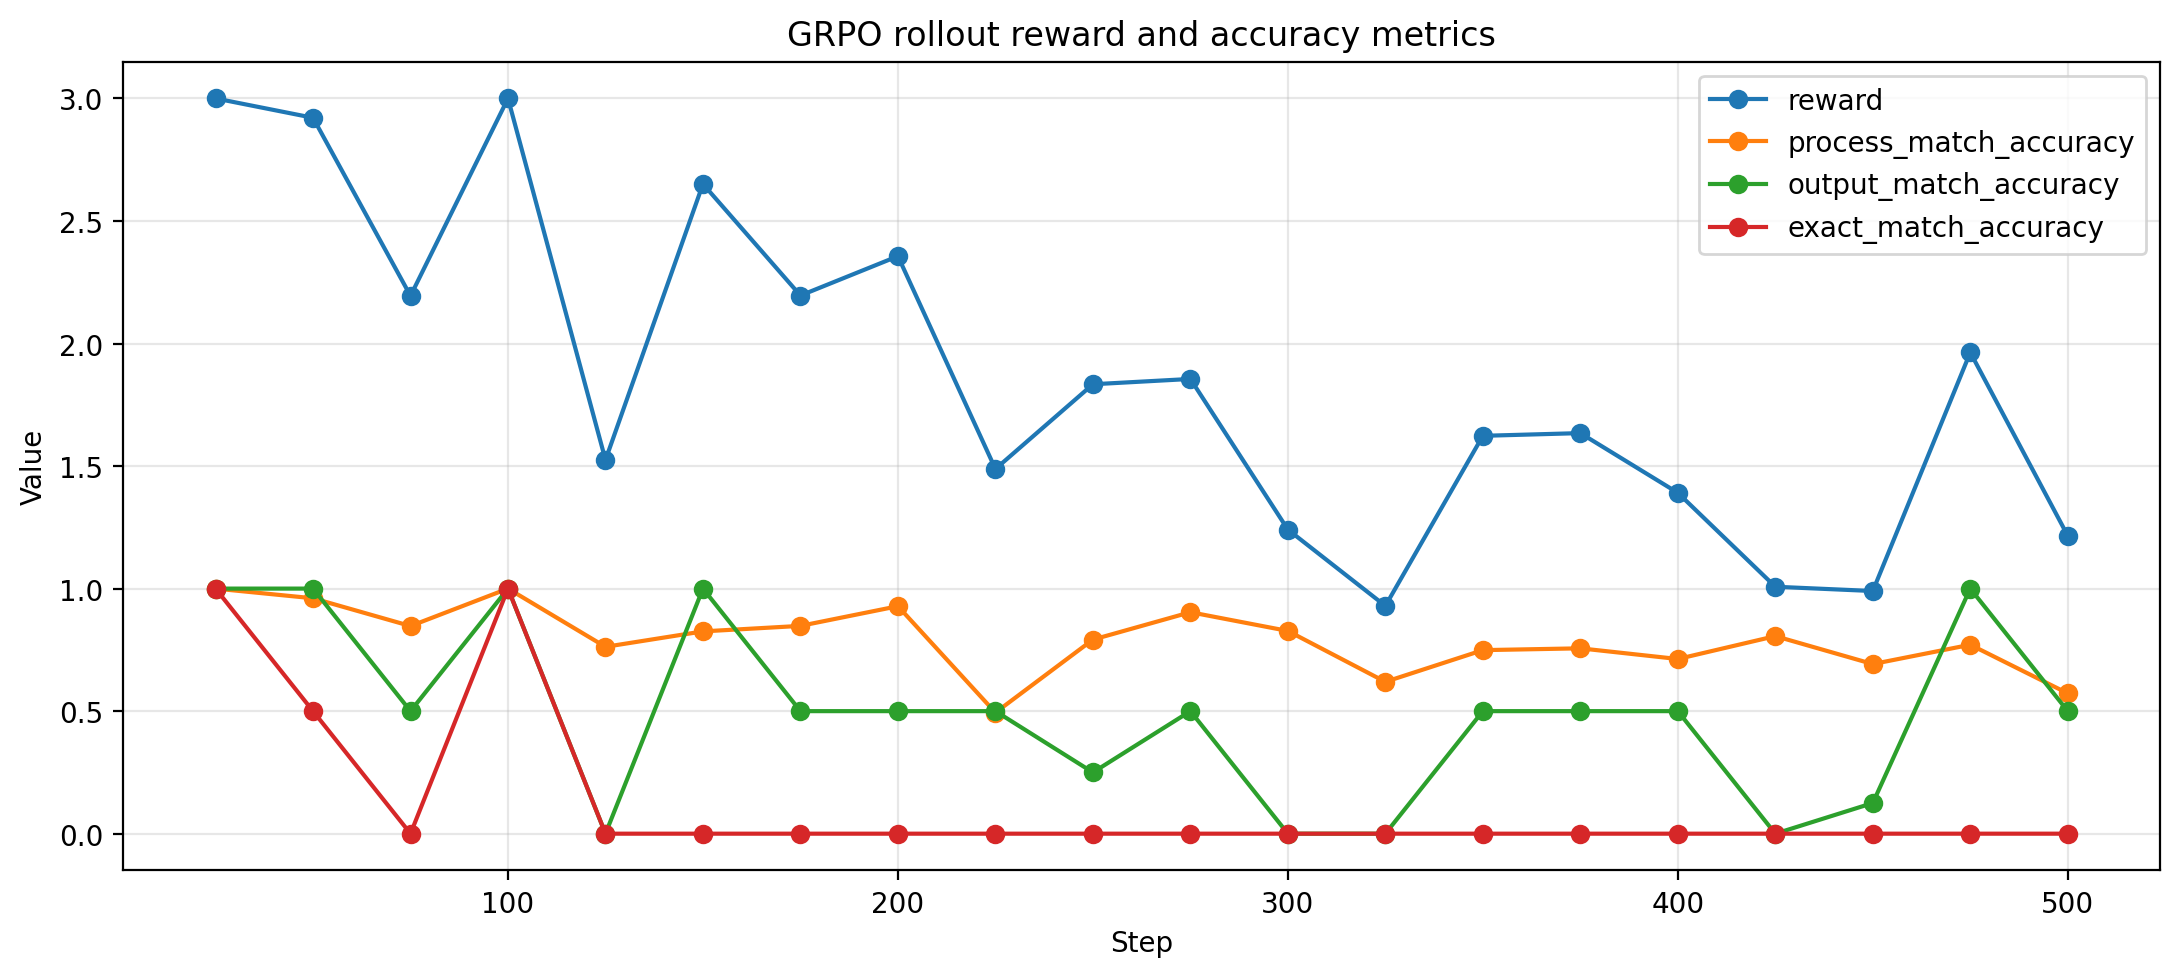
\includegraphics[width=0.96\linewidth]{01_grpo_rollout_reward_accuracy.png}
  \caption{GRPO rollout reward and accuracy metrics. The rollout metrics are noisy because each logged point is based on a small rollout batch, but they show that exact-match accuracy collapses when the curriculum reaches harder boundary lengths.}
  \label{fig:rollout_reward_accuracy}
\end{figure}

Figure~\ref{fig:loss_entropy} shows that the policy loss remains close to zero for much of training, while entropy generally increases from about 0.028 to 0.144. This suggests that the model continues to sample nontrivial alternatives, but the GRPO update signal may be weak or unstable. One possible explanation is low reward variance within the small GRPO groups, which can make group-relative advantages small or noisy.

\begin{figure}[H]
  \centering
  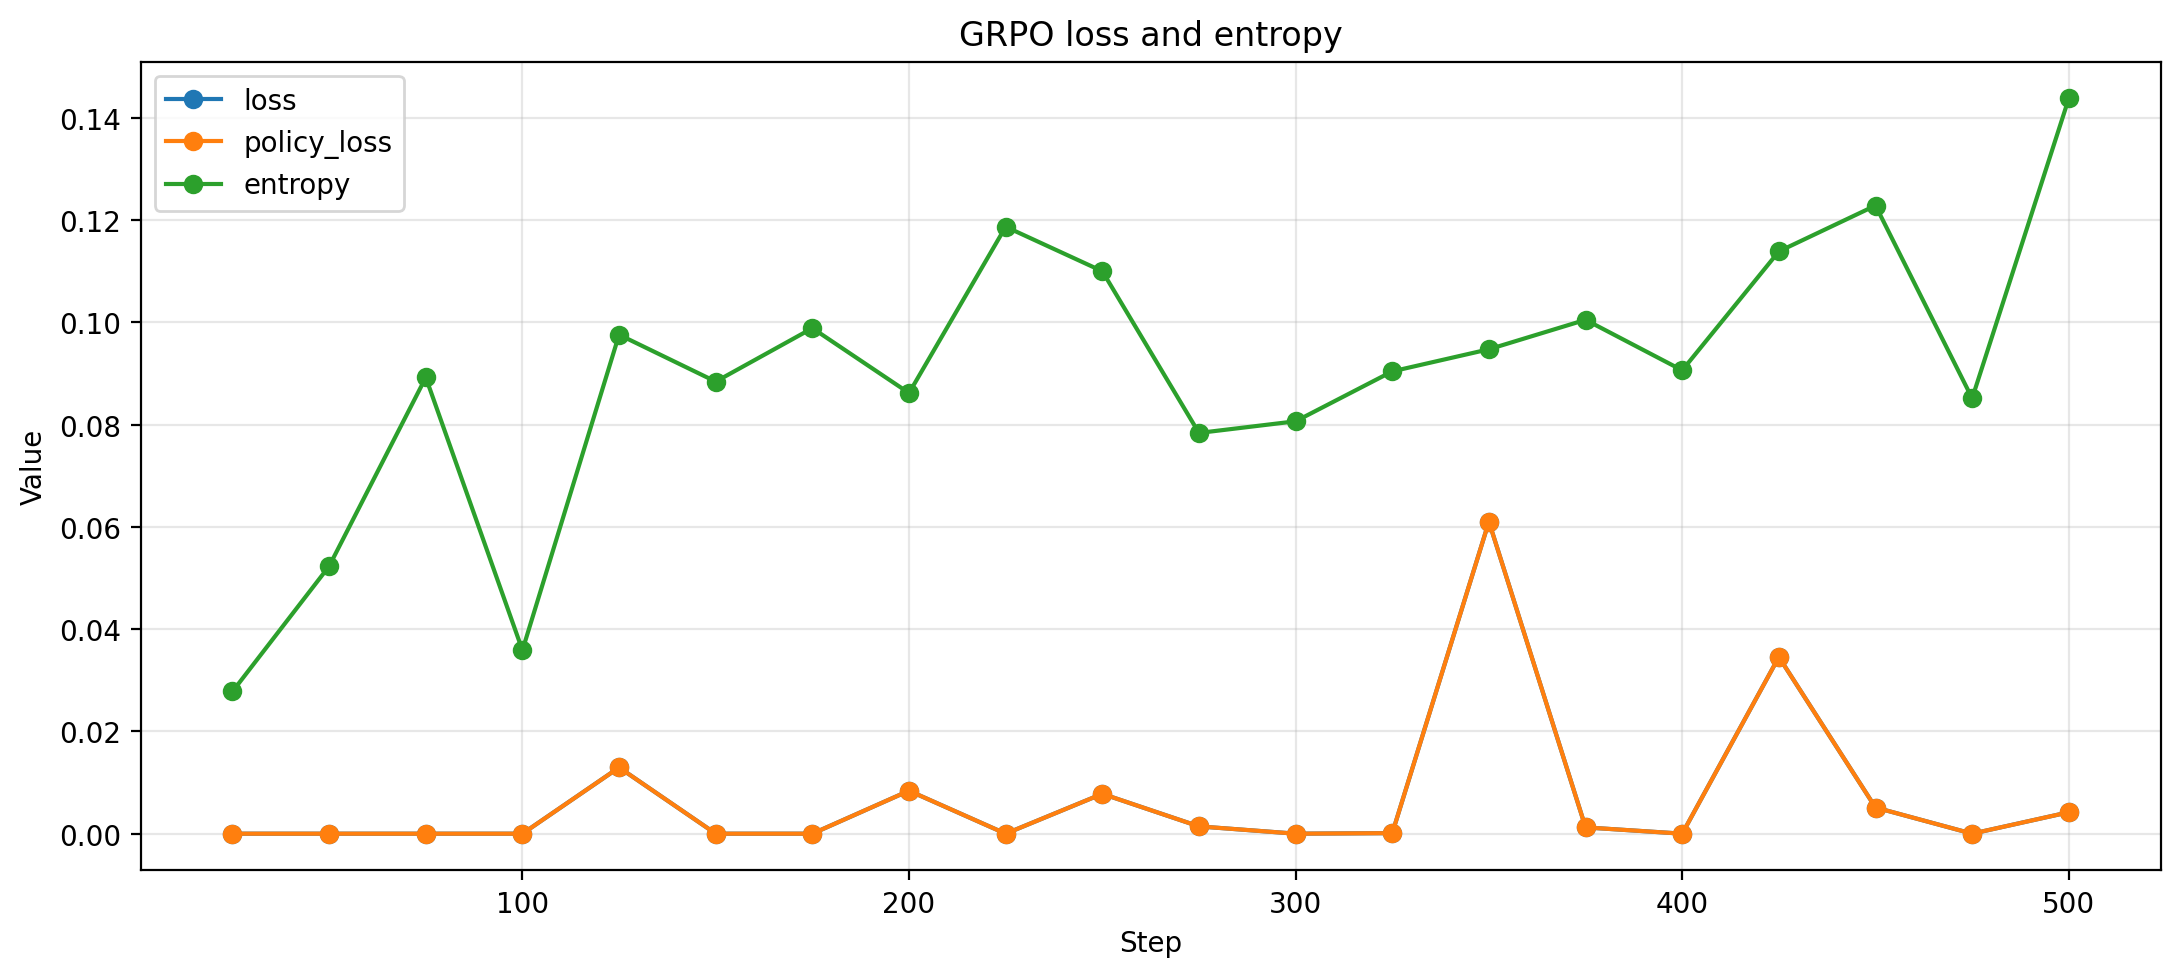
\includegraphics[width=0.96\linewidth]{02_grpo_loss_entropy.png}
  \caption{GRPO loss and entropy. Entropy increases over training, while the policy loss is often near zero, indicating that the optimization signal is not consistently strong.}
  \label{fig:loss_entropy}
\end{figure}

Figure~\ref{fig:tokens_curriculum} summarizes generation length and curriculum behavior. The mean generated token count increases as the curriculum moves to longer examples. This is expected because the trace length scales with input length, but it also increases the probability of formatting errors and exact-match failures.

\begin{figure}[H]
  \centering
  \begin{subfigure}{0.49\linewidth}
    \centering
    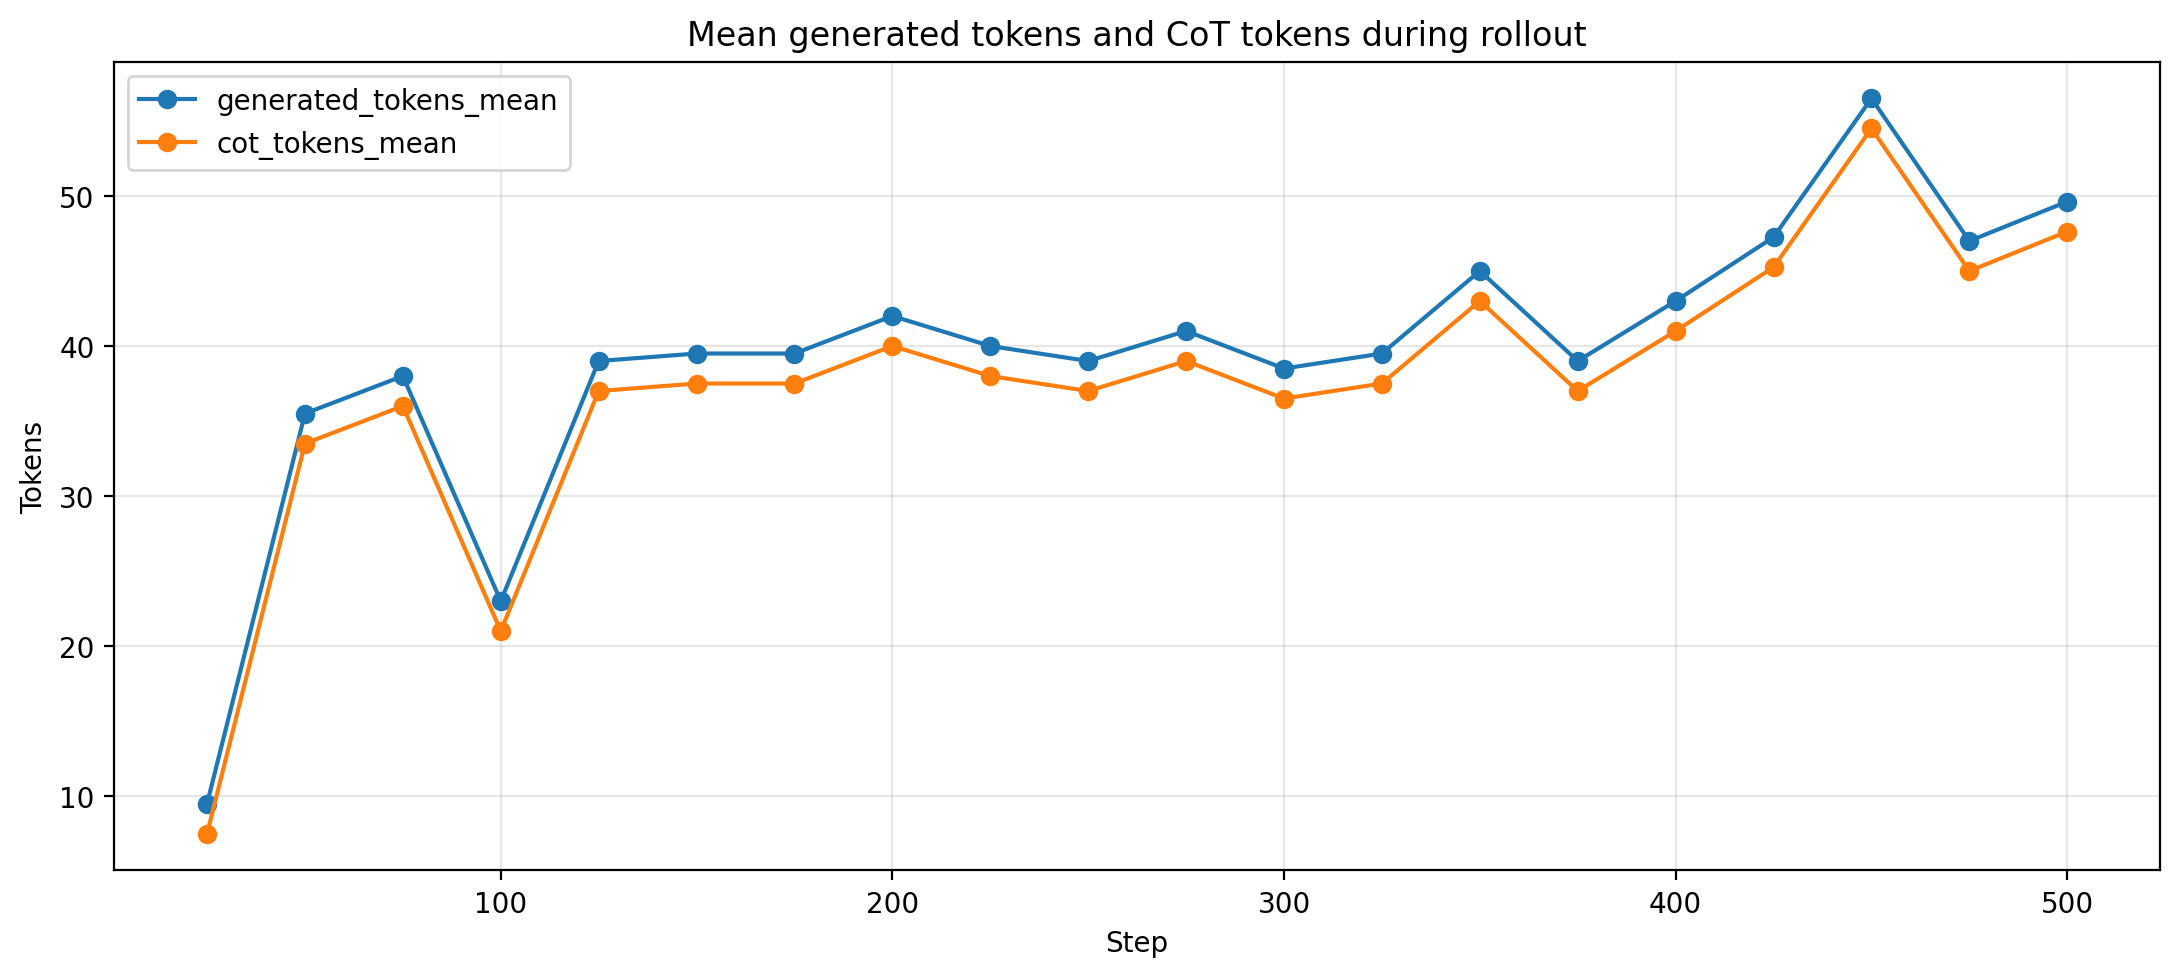
\includegraphics[width=\linewidth]{03_rollout_generated_and_cot_tokens.png}
    \caption{Generated and CoT token counts}
  \end{subfigure}
  \hfill
  \begin{subfigure}{0.49\linewidth}
    \centering
    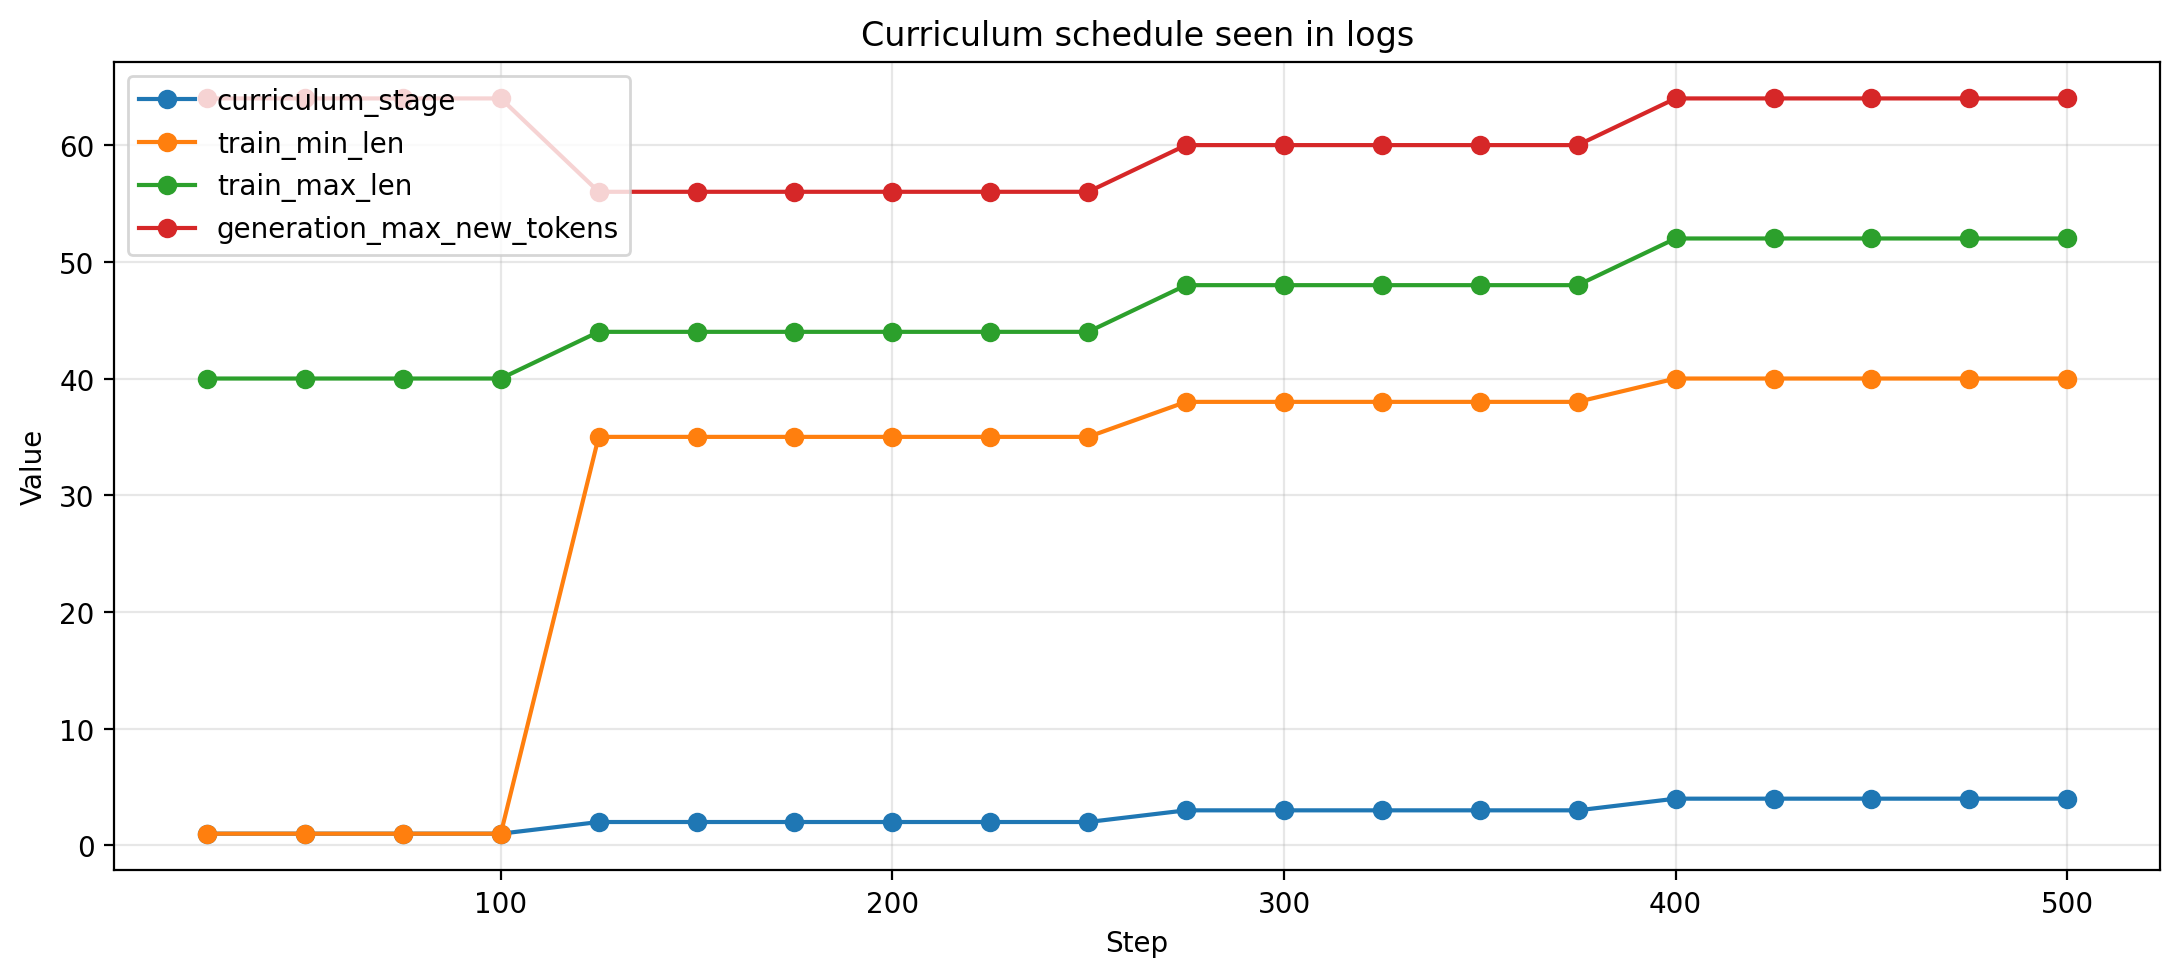
\includegraphics[width=\linewidth]{04_curriculum_schedule.png}
    \caption{Curriculum schedule}
  \end{subfigure}
  \caption{Generation length and curriculum schedule. The later curriculum stages sample boundary lengths near and beyond 40, increasing sequence length and difficulty.}
  \label{fig:tokens_curriculum}
\end{figure}

\section{Evaluation Results}
The evaluation metrics separate process accuracy, terminal accuracy, and exact-match accuracy. This separation is important because a model can partially learn the intermediate state transition while still failing to produce the exact full trace or final answer.

\begin{table}[H]
\centering
\caption{Final SFT vs. GRPO comparison at the last logged GRPO checkpoint. Positive deltas mean GRPO is better than SFT.}
\label{tab:final_comparison}
\begin{tabular}{llrrr}
\toprule
Bucket & Metric & SFT & GRPO final & Delta \\
\midrule
OOD 41--80 & Process & 0.5261 & 0.5603 & +0.0341 \\
OOD 41--80 & Terminal & 0.4750 & 0.3750 & -0.1000 \\
OOD 41--80 & Exact & 0.0000 & 0.0000 & +0.0000 \\
Train 1--40 & Process & 0.9683 & 0.9705 & +0.0021 \\
Train 1--40 & Terminal & 0.8750 & 0.8250 & -0.0500 \\
Train 1--40 & Exact & 0.7750 & 0.7250 & -0.0500 \\
\bottomrule
\end{tabular}
\end{table}

\subsection{Process Accuracy}
Figure~\ref{fig:eval_process} shows the strongest positive signal in the current run. GRPO maintains very high process accuracy on the train bucket and slightly improves OOD process accuracy over SFT. At the final checkpoint, OOD process accuracy reaches 0.5603 compared with 0.5261 for SFT, a gain of about 3.4 percentage points.

\begin{figure}[H]
  \centering
  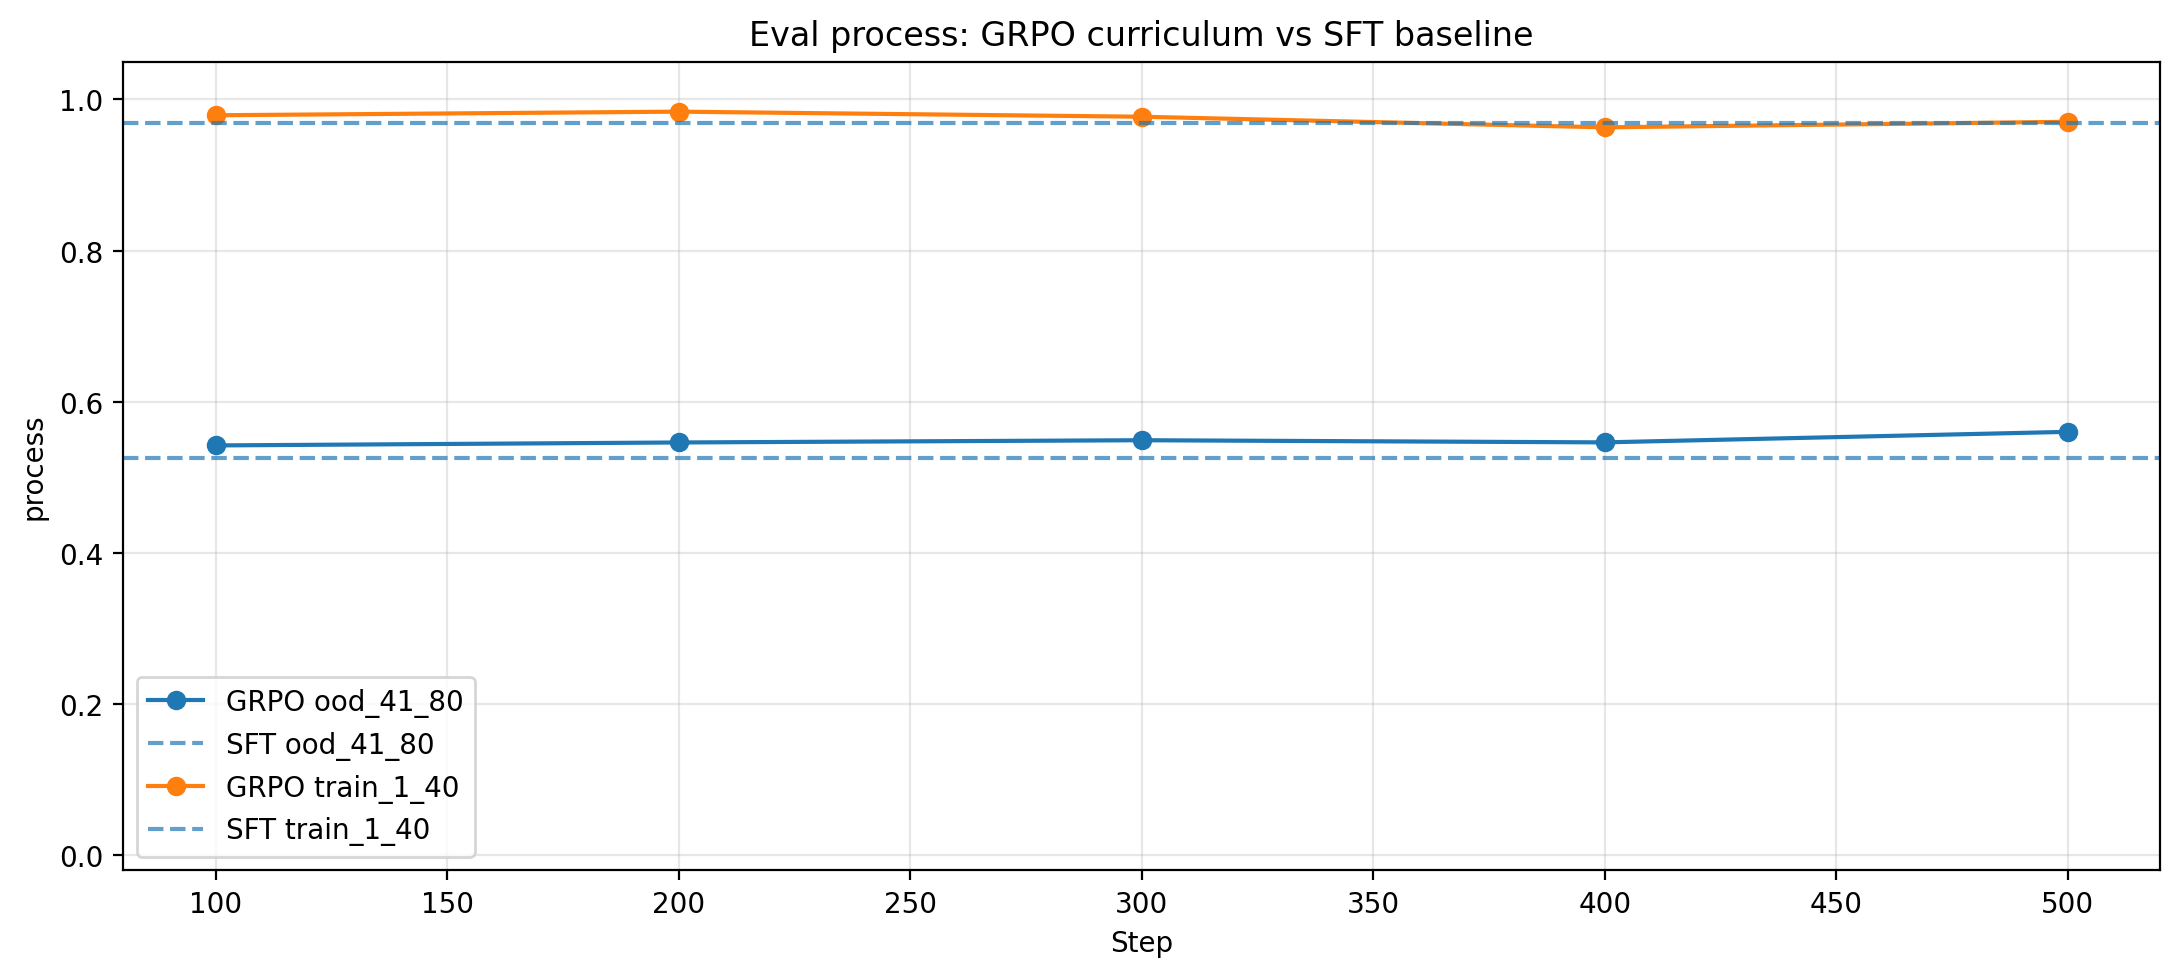
\includegraphics[width=0.96\linewidth]{05_eval_process_by_length_bucket.png}
  \caption{Evaluation process accuracy. GRPO slightly improves OOD process accuracy over the SFT baseline, but the absolute OOD process score remains far below the in-distribution score.}
  \label{fig:eval_process}
\end{figure}

\subsection{Terminal Accuracy}
Figure~\ref{fig:eval_terminal} shows that the process improvement does not transfer to final-answer accuracy. At the final checkpoint, OOD terminal accuracy is 0.3750 for GRPO compared with 0.4750 for SFT. Train terminal accuracy also decreases from 0.8750 for SFT to 0.8250 for GRPO.

\begin{figure}[H]
  \centering
  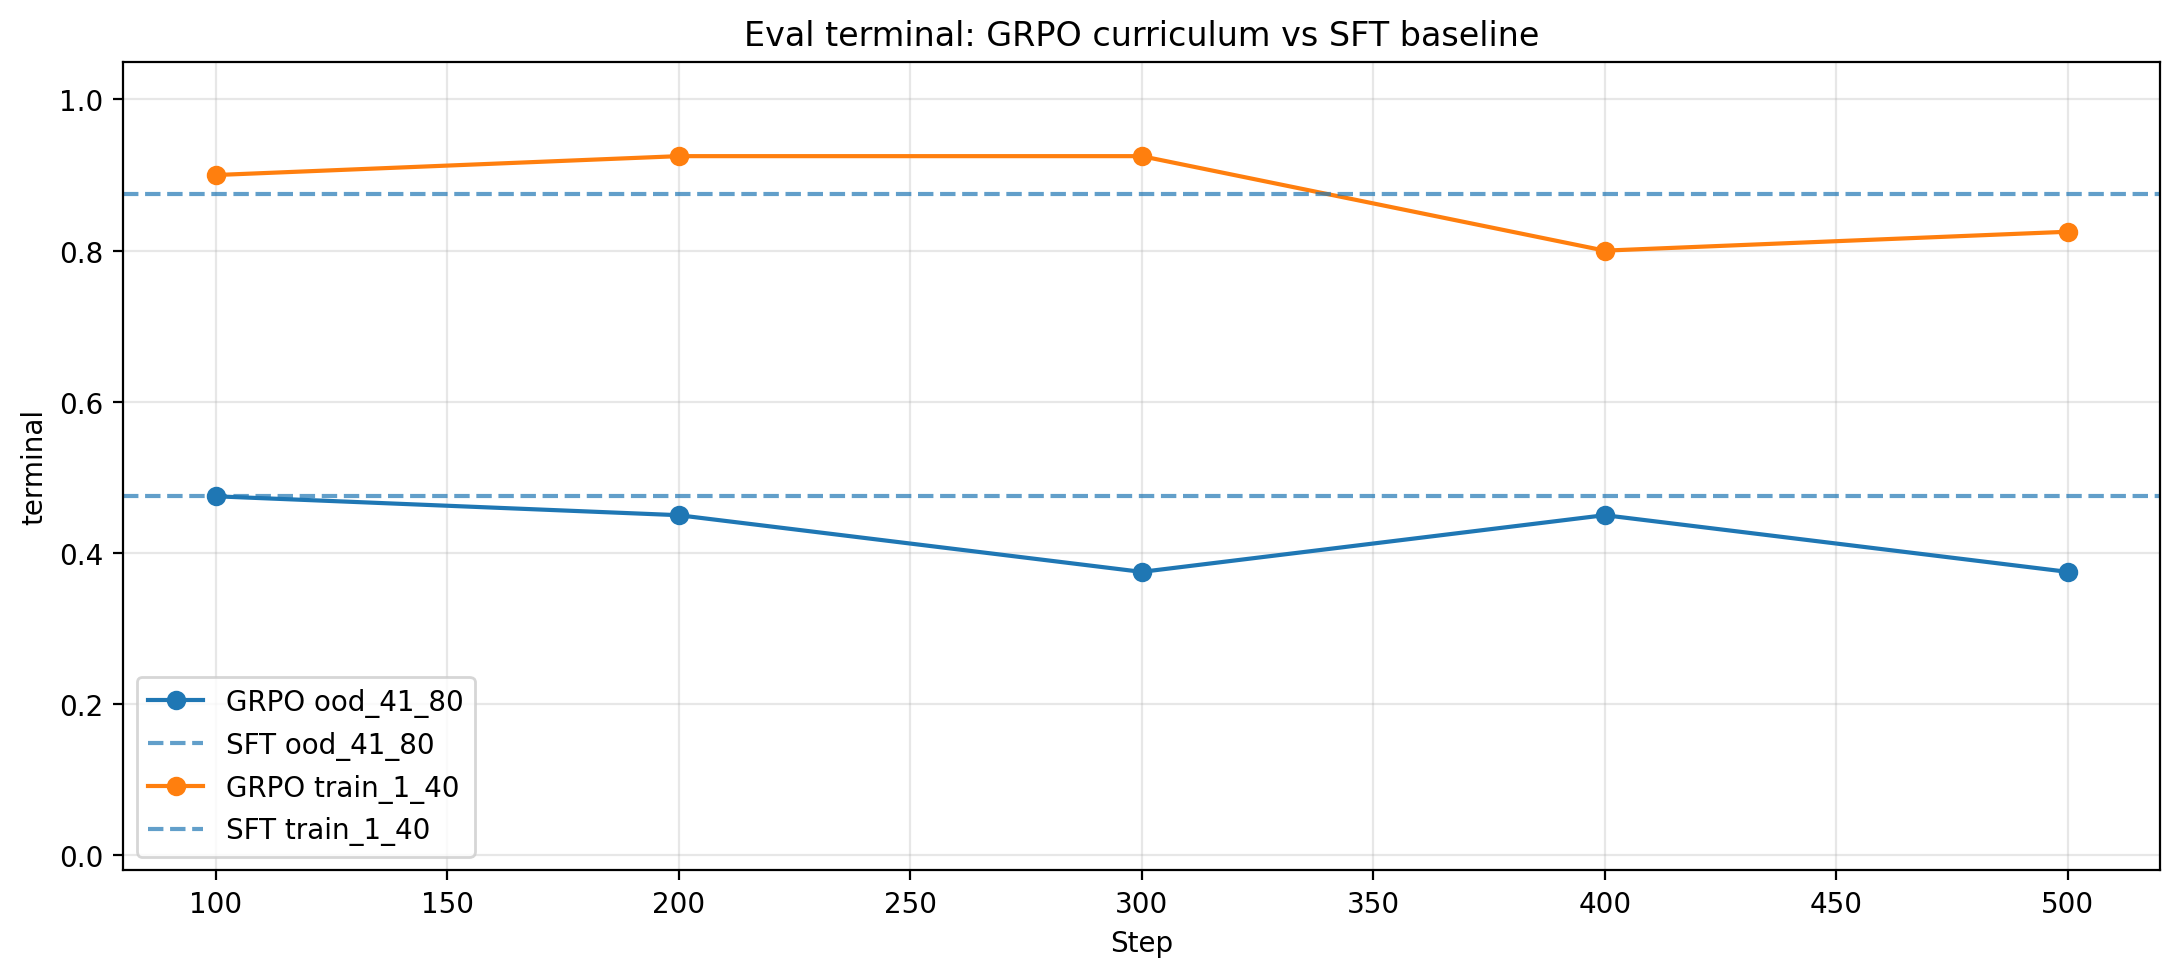
\includegraphics[width=0.96\linewidth]{05_eval_terminal_by_length_bucket.png}
  \caption{Evaluation terminal accuracy. GRPO does not improve terminal accuracy in the current run; final OOD terminal accuracy is lower than the SFT baseline.}
  \label{fig:eval_terminal}
\end{figure}

\subsection{Exact-Match Accuracy}
Exact match is the strictest metric because the entire generated trace and final answer must match the oracle output. Figure~\ref{fig:eval_exact} shows that in-distribution exact match remains moderate, but OOD exact match is zero for both SFT and GRPO. This is the clearest evidence that the current run has not yet solved length generalization.

\begin{figure}[H]
  \centering
  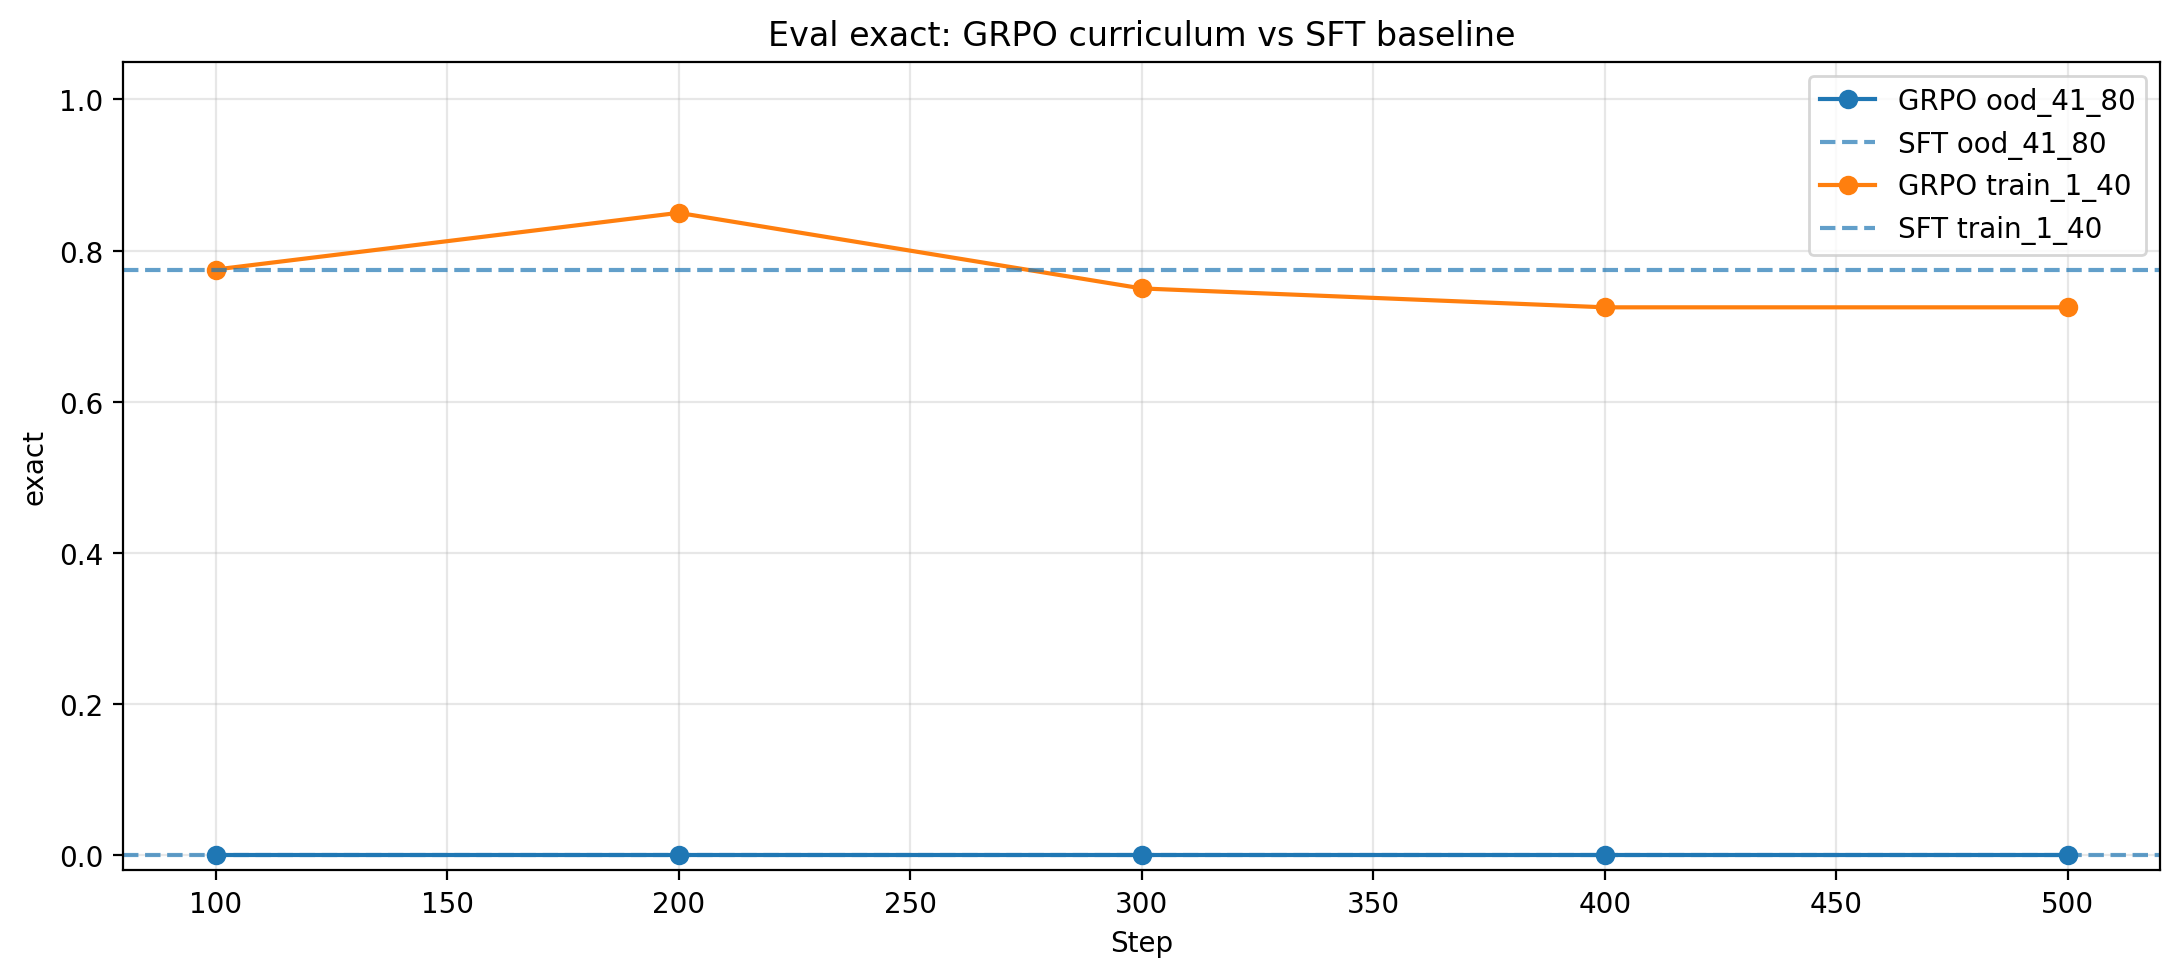
\includegraphics[width=0.96\linewidth]{05_eval_exact_by_length_bucket.png}
  \caption{Evaluation exact-match accuracy. OOD exact match remains 0.0000 throughout the logged checkpoints, indicating no robust exact trace generalization to lengths 41--80.}
  \label{fig:eval_exact}
\end{figure}

\section{Final Comparison Plots}
Figure~\ref{fig:final_comparison_plots} summarizes the final SFT versus GRPO comparison. The process metric is the only metric with a positive GRPO delta. Terminal and exact-match metrics are worse or unchanged.

\begin{figure}[H]
  \centering
  \begin{subfigure}{0.32\linewidth}
    \centering
    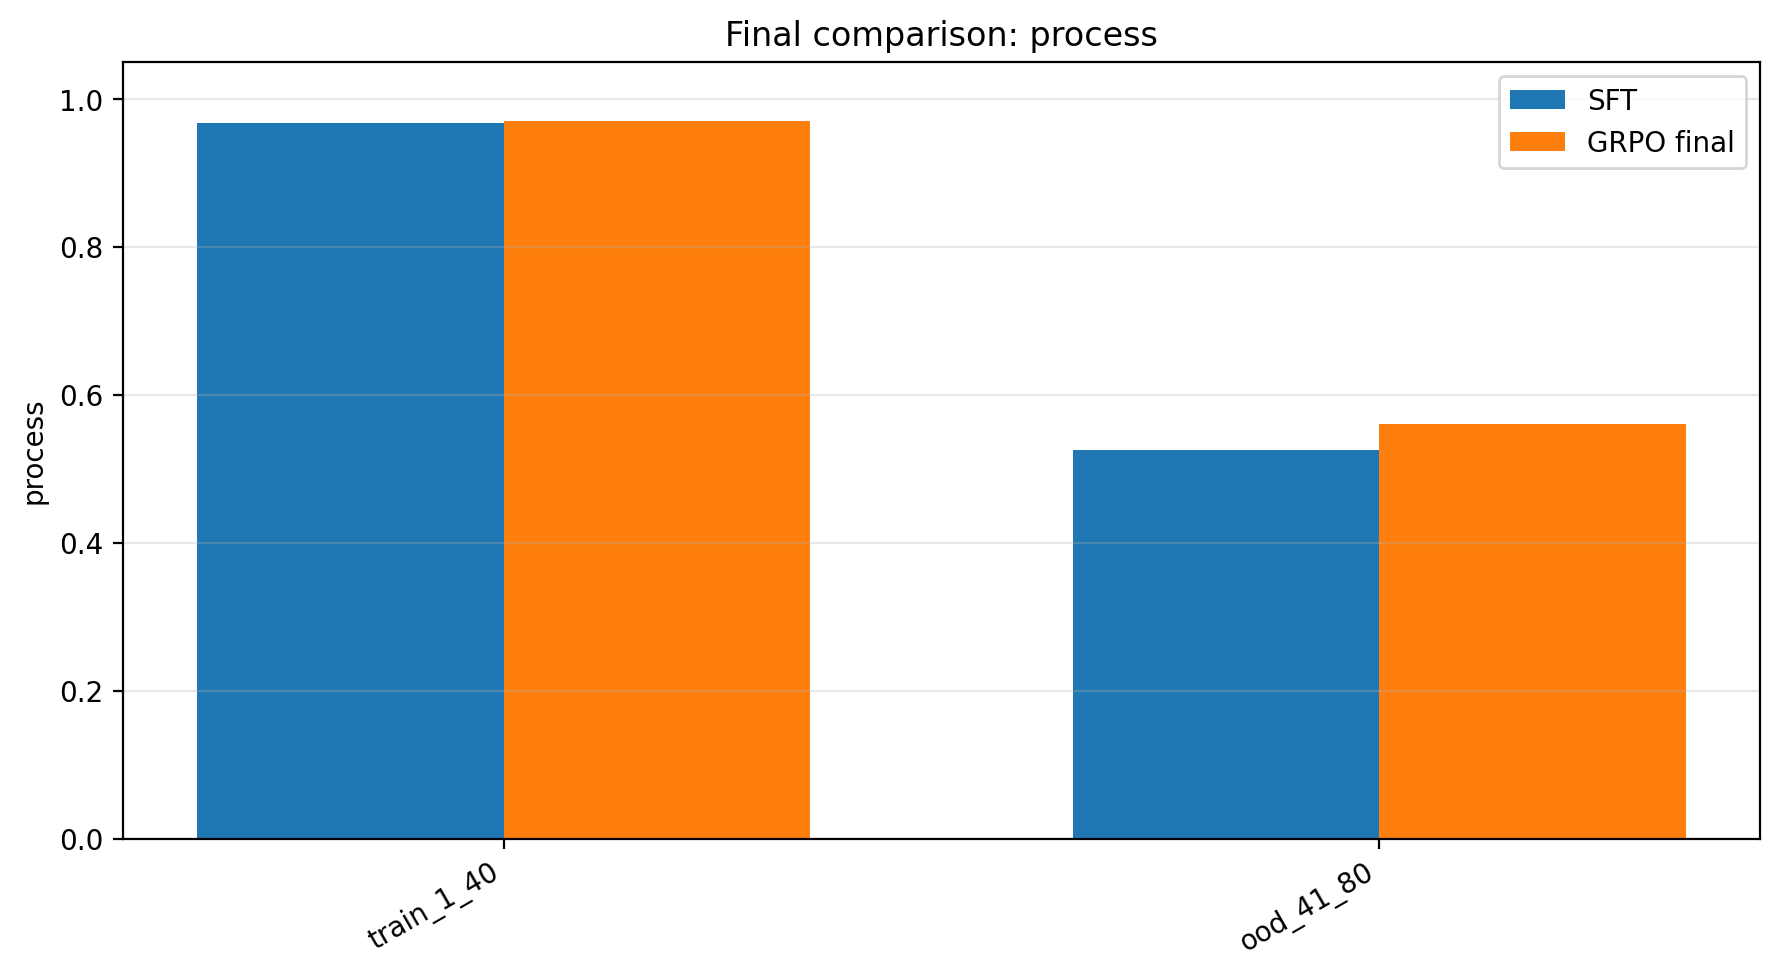
\includegraphics[width=\linewidth]{06_final_sft_vs_grpo_process.png}
    \caption{Process}
  \end{subfigure}
  \hfill
  \begin{subfigure}{0.32\linewidth}
    \centering
    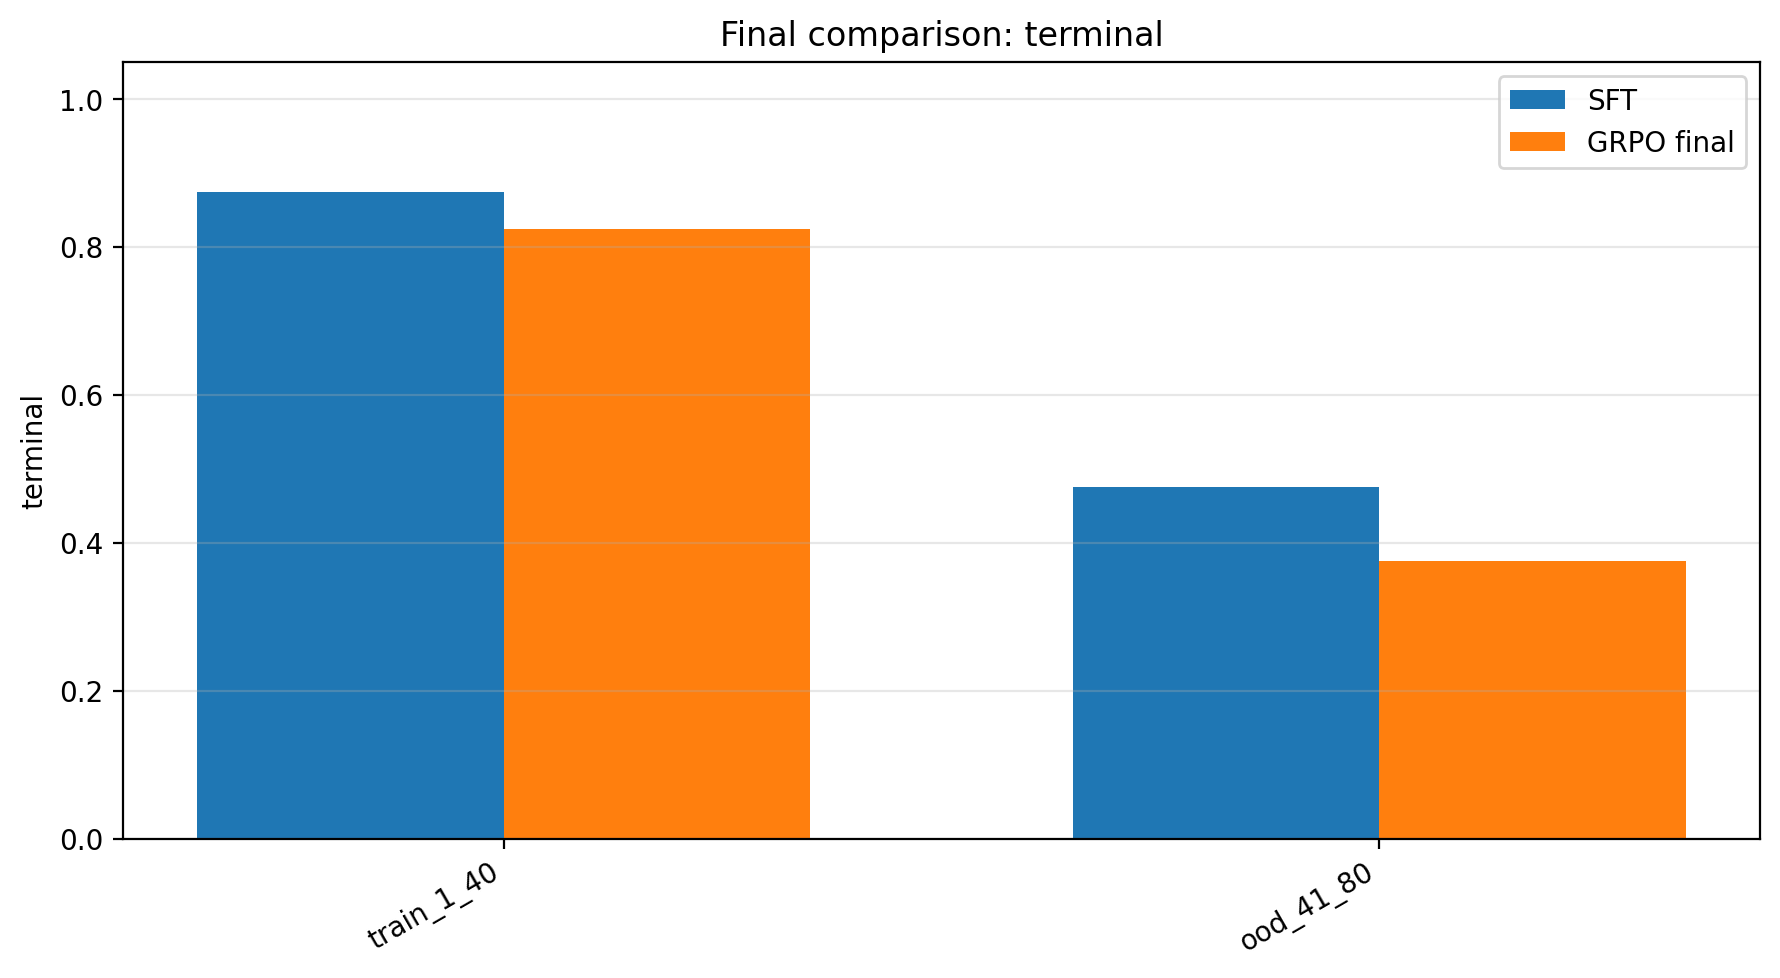
\includegraphics[width=\linewidth]{06_final_sft_vs_grpo_terminal.png}
    \caption{Terminal}
  \end{subfigure}
  \hfill
  \begin{subfigure}{0.32\linewidth}
    \centering
    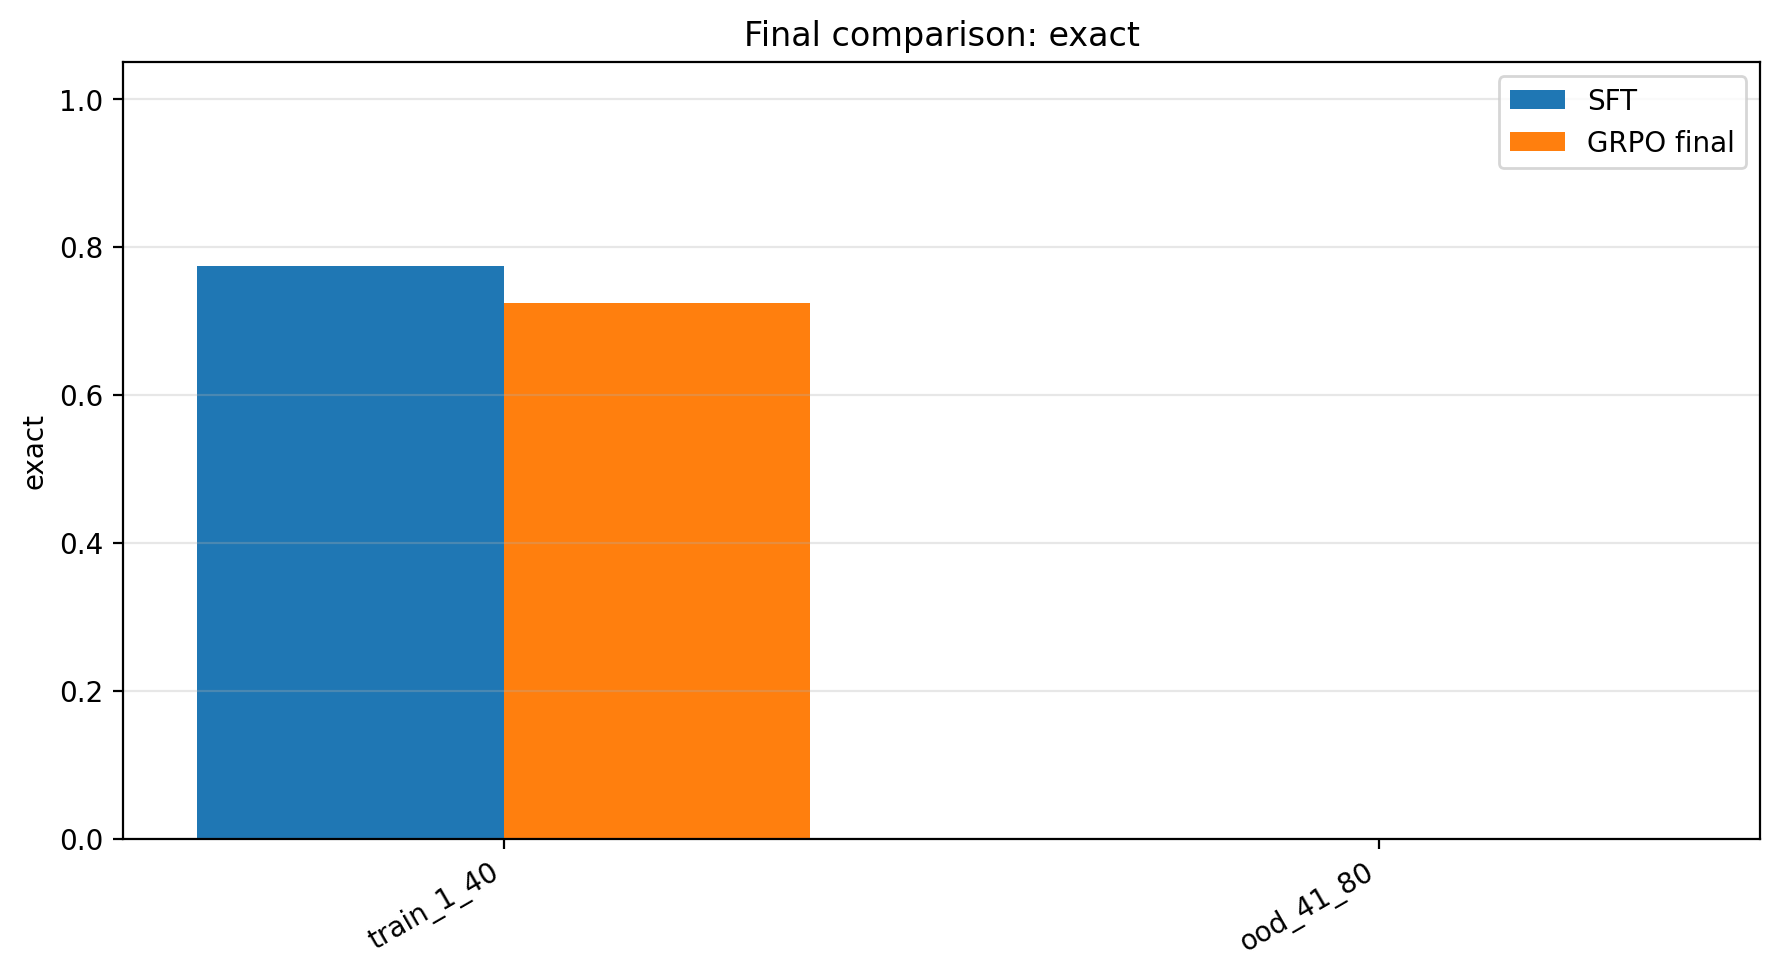
\includegraphics[width=\linewidth]{06_final_sft_vs_grpo_exact.png}
    \caption{Exact}
  \end{subfigure}
  \caption{Final SFT versus GRPO comparison. GRPO improves OOD process accuracy slightly, but does not improve terminal or exact-match accuracy.}
  \label{fig:final_comparison_plots}
\end{figure}

\section{Key Findings}
The main findings from the notebook are as follows.
\begin{enumerate}[leftmargin=*]
  \item \textbf{The process reward gives a measurable but small OOD process-accuracy gain.} Final OOD process accuracy improves from 0.5261 under SFT to 0.5603 under GRPO. This suggests that the intermediate reward is pushing the model toward better local parity-state tracking.
  \item \textbf{The process gain does not yet translate into better final answers.} OOD terminal accuracy decreases from 0.4750 to 0.3750 at the final GRPO checkpoint. Therefore, the current GRPO run improves one diagnostic metric while hurting the metric that determines final task success.
  \item \textbf{Exact length generalization is not achieved.} OOD exact match remains 0.0000 for both SFT and GRPO. This means the model is not generating fully correct longer traces and final answers for lengths 41--80.
  \item \textbf{In-distribution performance remains much stronger than OOD performance.} Final train-bucket process accuracy is 0.9705, but final OOD process accuracy is only 0.5603. This large gap indicates that the model still depends heavily on the training-length regime.
  \item \textbf{Curriculum difficulty strongly affects rollout stability.} Early logs show near-perfect rollout scores, but later boundary-length curriculum stages cause exact-match rollout accuracy to collapse. This suggests that the model can handle short cases but is brittle when trace length increases.
\end{enumerate}

\section{Interpretation}
The results support the motivation for process supervision, but only partially. The positive OOD process delta shows that intermediate rewards can improve the model's trace-level behavior. However, the lack of terminal and exact-match improvement means the current training setup is not sufficient for reliable algorithmic generalization.

A likely issue is that the model can receive partial process credit without learning a fully consistent parity algorithm across the entire generated sequence. For parity, a single early state error flips the downstream state sequence. The process score can still remain above random if many positions match locally, but exact match requires every state and the final output to be correct. This explains why the process metric can improve while exact match remains zero.

Another issue is formatting and sequence-length brittleness. As input length grows, the model must generate a longer trace with the correct number of states and the correct final token. Even when the model has partially learned the transition rule, small formatting deviations can destroy exact-match accuracy.

\section{Limitations of the Current Run}
The current results should be viewed as preliminary. The notebook output contains one parity run with evaluation through step 500 and only the first OOD bucket, 41--80. It does not yet include full evaluation for 81--160, 161--320, or 321--500 in the uploaded analysis bundle. The logged rollout batch size is also small, so rollout curves should be interpreted as diagnostics rather than definitive performance estimates. Finally, the current GRPO run appears to improve process accuracy but not terminal or exact-match performance, so it should not be presented as a successful length-generalization result yet.

\section{Recommended Next Experiments}
The next stage should focus on converting the process-level improvement into terminal and exact-match gains.
\begin{enumerate}[leftmargin=*]
  \item \textbf{Run longer GRPO training with more evaluation checkpoints.} The final checkpoint may not be sufficient to determine whether terminal accuracy can recover after process accuracy improves.
  \item \textbf{Evaluate all OOD buckets.} The project goal includes lengths up to 500, so the evaluation should include 41--80, 81--160, 161--320, and 321--500.
  \item \textbf{Compare reward weights.} Since process accuracy improves but terminal accuracy drops, run ablations such as $(w_p,w_t)=(1,1)$, $(2,1)$, and $(1,2)$.
  \item \textbf{Increase GRPO group size.} Larger groups may give more reliable group-relative advantages and reduce noisy updates.
  \item \textbf{Add format-constrained decoding or stricter trace templates.} This would separate algorithmic failures from formatting failures and may improve exact-match reliability.
  \item \textbf{Track first-error position.} For parity, analyzing where the first trace error occurs would show whether failures are caused by early transition mistakes, late drift, or output formatting.
\end{enumerate}

\section{Conclusion}
The current parity GRPO experiment provides useful evidence about the strengths and weaknesses of process-based RL for formal-language length generalization. The most important positive result is that GRPO improves OOD process accuracy over the SFT baseline. However, this improvement is not enough to improve terminal accuracy or exact-match accuracy. Therefore, the current result should be reported as a preliminary diagnostic finding: process rewards help the model partially track intermediate states, but further work is needed to make this translate into reliable long-length algorithmic generalization.

\appendix
\section{Appendix: Raw Final Training Snapshot}
At step 500, the final logged rollout snapshot is:
\begin{table}[H]
\centering
\caption{Final logged rollout snapshot at step 500.}
\begin{tabular}{lr}
\toprule
Metric & Value \\
\midrule
Reward & 1.2156 \\
Process match accuracy & 0.5725 \\
Output match accuracy & 0.5000 \\
Exact match accuracy & 0.0000 \\
Generated tokens mean & 49.6250 \\
CoT tokens mean & 47.6250 \\
\bottomrule
\end{tabular}
\end{table}

\section{Appendix: Best OOD Checkpoints}
For the first OOD bucket, 41--80, the best observed terminal score is 0.4750 at step 100, the best process score is 0.5603 at step 500, and exact match remains 0.0000 at all logged evaluation checkpoints. This again shows that process-level improvement and final-answer improvement are not yet aligned.

\end{document}
